%!TEX root = ../thesis.tex

\subsection{閾値による因果順序の推定精度の影響}

提案アルゴリズムは、式~\eqref{alg:MRS}による
モーメント比スコア$\widehat{\mathcal S}(m,j)$が閾値より小さいかどうかによって
離散変数と連続変数の因果順序を推定している。
そのため、閾値の設定が因果順序の推定精度に影響を与える。
そこで本節では、以下の数値実験を行うことで、
モーメント比スコアの閾値の設定によって因果順序の推定精度がどのように変化するのかを示す。

本節の数値実験では、
頂点数を$p = 5$、
連続変数の誤差変数の分布を一様分布に固定し、分散は$\sigma_j^2 = 0.75$とした。
また、因果順序が一意に定まるように、データ生成過程のグラフ構造は
図\ref{fig:threshold}とした。
四角形で表した頂点$X_1,X_3,X_5$に離散変数を割り当て、
各変数の条件付き分布はポアソン分布に従うこととした。
真の因果順序において、離散変数と連続変数が交互に現れるため、
閾値の設定が因果順序の推定精度に最も影響を与えると考えられる。
なお、サンプルサイズや各頂点間の関係性の強さのパラメータ$\theta_{jk}$、定数項$\theta_j$は、
\ref{subsection:setup}節に記載の内容と同じとした。

\begin{figure}[ht]
  \centering
  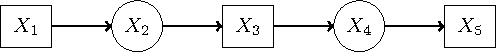
\includegraphics{./picture/threshold.pdf}
  \caption{閾値による因果順序の推定精度を測定する数値実験におけるグラフ構造}
  \label{fig:threshold}
\end{figure}

閾値は $ \{ 1.000, 1.002, \dots, 1.050 \}$とし、
それぞれ100回ずつデータ生成と因果順序の推定を繰り返した。
因果順序の推定精度は、正解率(Accuracy)によって測定した。
正解率の算出方法は以下の通りである。
\begin{itemize}
  \item 正解率(Accuracy)
  \begin{equation*}
    \frac{\text{因果順序が正しく推定された回数}}{\text{繰り返し回数}}
  \end{equation*}
\end{itemize}

\begin{figure}
  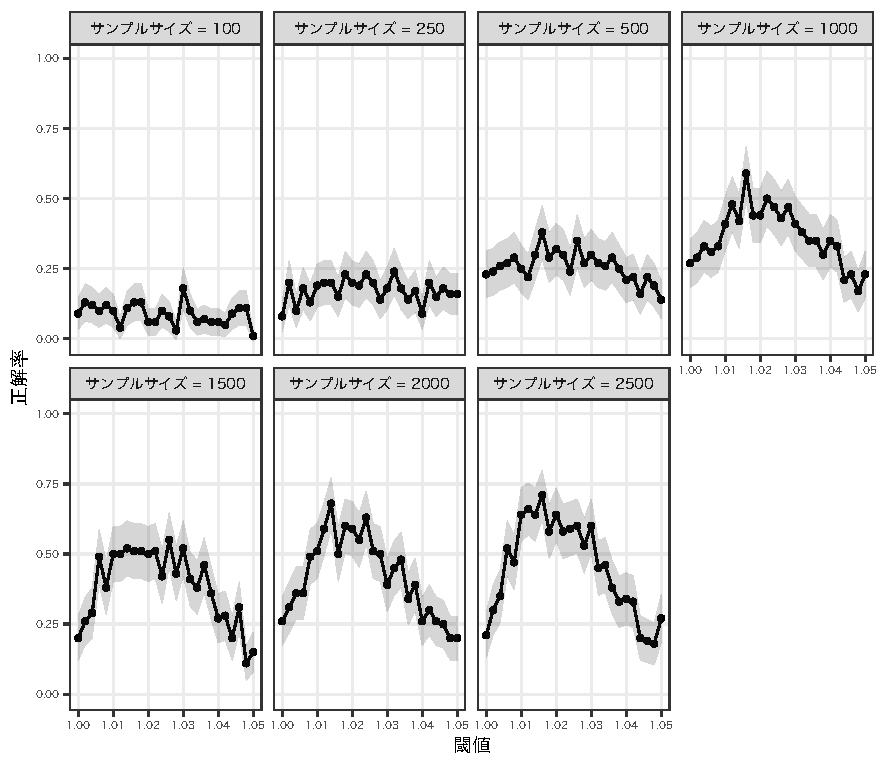
\includegraphics[width=13cm, bb=9 9 358 434]{./picture/plot_threshold.pdf}
  \caption{閾値の設定と因果順序の推定精度の関係}
  \label{fig:plot_threshold}
\end{figure}

数値実験の結果を図\ref{fig:plot_threshold}に示す。
サンプルサイズ$\{ 100, 200 \}$ではどの閾値でも正解率が0.25以下で、
閾値による因果順序の推定精度への影響は見られなかった。
一方、サンプルサイズ500以上では、閾値の範囲$[1.01, 1.02]$において正解率が高い。
つまり、離散変数と連続変数の因果順序を推定する際の閾値は、
範囲$[1.01, 1.02]$で設定することが望ましいと言える。
